\documentclass[aspectratio=169]{beamer}
\usepackage{graphicx}

\usetheme{default}

\graphicspath{{ .} }

\title{Federated Multicloud}
\subtitle{Common infrastructure services for NFDI}
\author{
	Marius Dieckmann\inst{1,2,3}\newline\url{Marius.Dieckmann@computational.bio.uni-giessen.de}
}

\institute[shortinst]{\textsuperscript{1} Justus-Liebig-Universität Gießen \and \inst{2} NFDI4Biodiversity \and \inst{3} de.NBI}

\begin{document}
	\begin{frame}[plain]
		\maketitle
	\end{frame}

	\begin{frame}{Federated Multicloud}
		\begin{figure}
			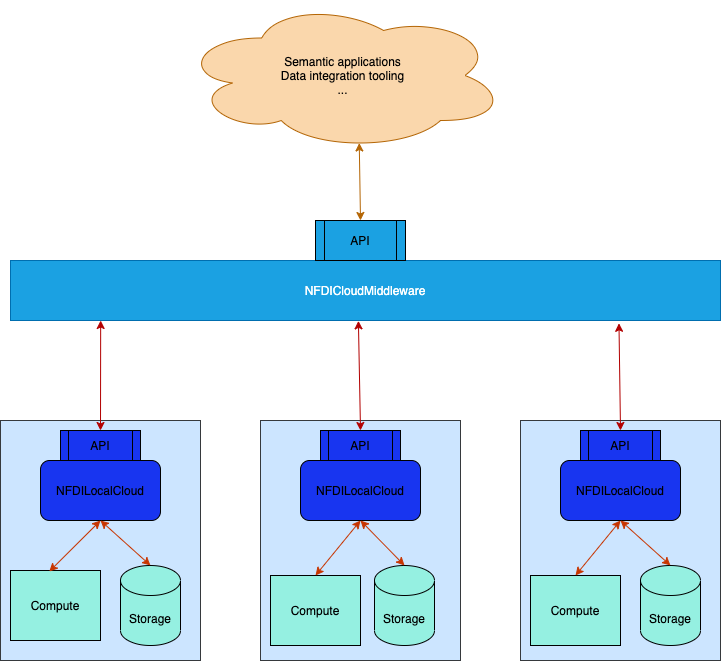
\includegraphics[scale=0.3]{../../images/WGMulticloudConcept.png}
		\end{figure}
	\end{frame}

	\begin{frame}{Basic concept}
		\begin{itemize}
				\item API based management system
				\item Local configurable deployments that are connected via a middleware across multiple datacenters
				\item Common AAI across all deployments
				\item gRPC API with pre-generated clients stubs
				\item HTTP-REST gateway with OpenAPI documentation
				\item Update event notification via event streaming
				\item gRPC API with pre-generated clients stubs
				\item HTTP-REST gateway with OpenAPI documentation
				\item Update event notification via event streaming
		\end{itemize}
	\end{frame}

	\begin{frame}{Components}
		\begin{itemize}
			\item Storage component:
			\begin{itemize}
				\item Simple data structure with consistent versioning
				\item Versioning schema based on semantic versioning
				\item Object history
				\item Configurable access rights for sensible data
				\item Update event notification via event streaming
				\item Caching and read-only (edge) deployments
			\end{itemize}
			\item Compute component:
			\begin{itemize}
				\item Various compute services
				\item Examples:
				\begin{itemize}
					\item Personal health train
					\item Cluster deployment (BiBiGrid)
					\item Simple website deployment (heroku)
				\end{itemize}
				\item List of available functions is provided by the local deployment (see GAIA-X)
			\end{itemize}
		\end{itemize}
	\end{frame}
	
	\begin{frame}{Implementation}
		\begin{itemize}
			\item Continous development based on continous requirements engineering
			\item Storage solution already in implementation in NFDI4Biodiv, NFDI4Microbiota and FAIR-datacenters
			\item Close cooperation with GAIA-X to reuse tooling if possible
			\item All components are containerized and designed to run in Kubernetes
			\item Components can be developed within the defined standards by individual subgroups
		\end{itemize}
	\end{frame}

	
	\end{document}